\documentclass{report}
\usepackage[T1]{fontenc} % Fontes T1
\usepackage[utf8]{inputenc} % Input UTF8
\usepackage[backend=biber, style=ieee]{biblatex} % para usar bibliografia
\usepackage{csquotes}
\usepackage[portuguese]{babel} %Usar língua portuguesa
\usepackage{blindtext} % Gerar texto automaticamente
\usepackage[printonlyused]{acronym}
\usepackage{hyperref} % para autoref
\usepackage{xcolor}
\usepackage{comment}
\usepackage{bchart}
\usepackage{caption}
\usepackage{graphicx}
\graphicspath{ {./images/} }
\usepackage{pgfplots}
\pgfplotsset{compat=1.15}
\newcommand{\lin}[1]{\centerline{\fbox{\texttt{#1}}}}

\bibliography{bibliografia}


\begin{document}
%%
% Definições
%
\def\titulo{Trabalho de Aprofundamento 2}
\def\data{Abril de 2019}
\def\autores{Miguel Cabral, David Bicho}
\def\autorescontactos{(93091) miguel.f.cabral@ua.pt, (93215) david23@ua.pt}
\def\versao{VERSAO}
\def\departamento{Departamento de Eletrónica, Telecomunicações e Informática}
\def\empresa{UA}
\def\logotipo{ua.pdf}
%
%%%%%% CAPA %%%%%%
%
\begin{titlepage}

\begin{center}
%
\vspace*{50mm}
%
{\Huge \titulo}\\ 
%
\vspace{10mm}
%
{\Large \empresa}\\
%
\vspace{10mm}
%
{\LARGE \autores}\\ 
%
\vspace{30mm}
%
\begin{figure}[h]
\center
\includegraphics{\logotipo}
\end{figure}
%
\vspace{30mm}
\end{center}
%
\begin{flushright}
\end{flushright}
\end{titlepage}

%%  Página de Título %%
\title{%
{\Huge\textbf{\titulo}}\\
{\Large \departamento\\ \empresa}
}
%
\author{%
    \autores \\
    \autorescontactos
}
%
\date{\data}
%
\maketitle

\pagenumbering{roman}

%%%%%% Agradecimentos %%%%%%
% Segundo glisc deveria aparecer após conclusão...
\renewcommand{\abstractname}{Agradecimentos}
\begin{abstract}
Neste trabalho queríamos agradecer aos docentes responsáveis pela \ac{uc} respetiva de cada aluno deste grupo ( A professora Pétia Georgieva e o Professor António Adrego) que lecionaram as aulas deste 2º semestre.
\end{abstract}


\tableofcontents
% \listoftables     % descomentar se necessário
% \listoffigures    % descomentar se necessário


%%%%%%%%%%%%%%%%%%%%%%%%%%%%%%%
\clearpage
\pagenumbering{arabic}

%%%%%%%%%%%%%%%%%%%%%%%%%%%%%%%%
\chapter{Introdução}
\label{chap.introducao}

Este trabalho foi realizado no âmbito da disciplina de Laboratórios de Informática.Este trabalho consiste em criar um programa cliente em python que fosse capaz de avaliar a qualidade de ligação ,especialmente latência e largura de banda de Download e Upload.\newline
O cliente irá aceder aos servidores que estão num ficheiro \ac{JSON} que foi fornecido pelos docentes.\newline
O cliente deverá efetuar testes periódicos usando múltiplos servidores. Ao longo da sua execução, deverá emitir um relatório, em formato \ac{CSV}, contendo os dados obtidos (report.csv).\newline
Os servidores utilizam o protocolo que opera sobre ligações \ac{TCP},efetuadas para o endereço e porta especificados no ficheiro servers.json.\newline
As mensagens trocadas são simples mensagens de texto terminadas pelo caractere'n'. 

Este documento está dividido em quatro capítulos.
Depois desta introdução,
no \autoref{chap.metodologia} é apresentada a metodologia seguida,
no \autoref{chap.resultados} são apresentados os resultados obtidos,
sendo estes discutidos no \autoref{chap.analise}.
Finalmente, no \autoref{chap.conclusao} são apresentadas
as conclusões do trabalho.

\chapter{Metodologia}
\label{chap.metodologia}
Descrição da forma de realização do trabalho e apresentação dos resultados.

\section{client.py}

\subsection{Funcionalidades}
O programa client.py tem como função de comunicar com o servidor através da leitura do ficheiro\ac{JSON} e criar um ficheiro \ac{CSV} com os resultados.


\subsection{Função valid()}
Esta função tem como principal objetivo verificar se os argumentos introduzidos no terminal são corretos.
Esta função vai realizar os seguintes passos:
\begin{itemize}
    \item Verificar se o cliente inicia o programa com um número de argumentos inferior a 3, se tal acontecer imprime no terminal uma mensagem.
    \item Verifica se é iniciado com argumentos inválidos (tipo errado, valor incorreto ou não encontrado),e apresenta uma mensagem de erro respetiva ao argumento que gera o erro.
\end{itemize}

\subsection{host()}
Esta função tem como objetivo:
\begin{itemize}
    \item Verificar se o 3 argumento introduzido é texto e se assim o for realizar o teste para qualquer servidor do país introduzido.
    \item Caso o 3 argumento for um número inteiro ,deverá realizar o teste para o servidor com esse identificador.
\end{itemize}

\subsection{main()}
Esta função realiza o seguinte:
\begin{itemize}
    \item O primeiro argumento introduzido deverá ser um número inteiro que irá indicar o intervalo em segundos entre cada teste.
    \item O segundo argumento deverá ser um número inteiro que irá indicar o número de testes que irão ser realizados.
\end{itemize}

\subsection{download()}
Esta função realiza o seguinte:
\begin{itemize}
    \item O cliente realiza uma descarga entre 10MB e 100MB ou até que passem 10 segundos.
    \item A taxa de largura de banda é calculada através do número de octetos recebidos sobre o tempo decorrido,após ter sido obtido 1MB.
\end{itemize}

\subsection{Ping()}
Esta função realiza o seguinte:
\begin{itemize}
    \item A latência deve ser calculada pelo tempo médio de 10 transações de PING/PONG.
\end{itemize}

\subsection{readJSON()}
Esta função realiza o seguinte:
\begin{itemize}
    \item Recebe o host e retorna o id desse host.
\end{itemize}

\subsection{Main()}
A Função Main realiza o seguinte:
\begin{itemize}
    \item Abre o ficheiro \ac{CSV} e,enquanto o número de testes for inferior ao argumento introduzido, escreve neste os resultados obtidos.
\end{itemize}

\chapter{Resultados}
\label{chap.resultados}
Neste capítulo vamos mostrar alguns testes que foram realizados com erros induzidos por nós ,para mostrar o resultado no terminal esperado.
\section{Erro de argumentos}
Quando o número de argumentos não é o correto ou não é adequado o resultado no terminal é o mostrado na figura 3.1 :
\begin{figure}
    \centering
    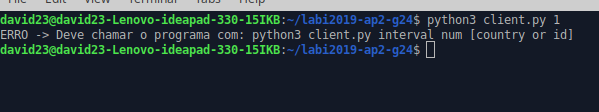
\includegraphics[width=13cm]{argumento.png}
    \caption{Erro de argumentos}
    \label{argumentos}
\end{figure}
\section{Comparação de Ping}
Nas figuras 3.2 podemos comparar o PING em Portugal e na China.O resultado é o esperado visto que o PING é muito superior na China do que em Portugal,visto que o servidor está mais distante.
\begin{figure}
    \centering
    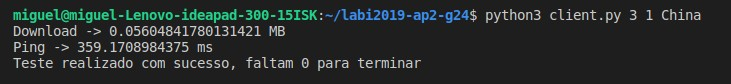
\includegraphics[width=13cm]{China.jpeg}
    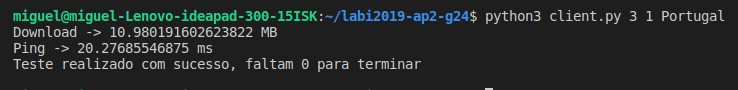
\includegraphics[width = 13cm]{Portugal.jpeg}
    \caption{Comparação de Ping}
    \label{fig:my_label}
\end{figure}
\section{País ou Id inválido}
Quando o país ou o Id introduzido como argumento é inválido o resultado no Output é o mostrado na figura 3.3 :
\begin{figure}
    \centering
    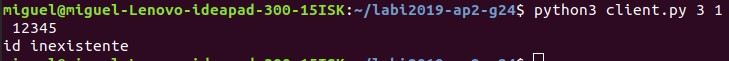
\includegraphics[width = 13 cm]{idinvalido.jpg}\newline
    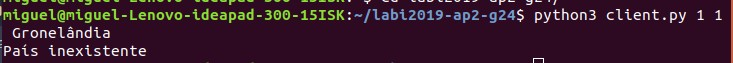
\includegraphics[width = 13cm]{gronelandia.jpg}
    \caption{figura 3.4}
    \label{fig:my_label}
\end{figure}
\section{Report.csv}
Quando todos os argumentos introduzidos são os esperados ,é escrito os valores do Contador,id do servidor,data e hora no formato ISO,latência,largura de banda,check,como mostra a figura 3.4 :
\begin{figure}
    \centering
    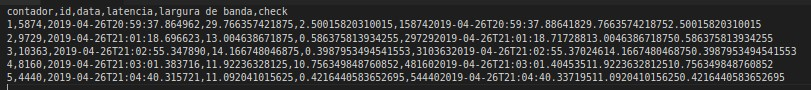
\includegraphics[width=13cm]{csv.jpg}
    \caption{figura 3.4}
    \label{fig:my_label}
\end{figure}
\chapter{Conclusões}
\label{chap.conclusao}
Este trabalho permitiu ao grupo aprofundar os conhecimentos sobre python e sobre a implementação de sockets e manipulação de ficheiros \ac{JSON}.

\chapter*{Contribuições dos autores}
David Bicho 50\%
Miguel Cabral 50\%

%%%%%%%%%%%%%%%%%%%%%%%%%%%%%%%%%
\chapter*{Acrónimos}
\begin{acronym}
\acro{ua}[UA]{Universidade de Aveiro}
\acro{CSV}{Comma Separated Values}
\acro{TCP}{ Transmission Control Protocol}
\acro{JSON}[JSON]{JavaScript Object Notation}
\acro{uc}{Unidade Curricular}
\acro{miect}[MIECT]{Mestrado Integrado em Engenharia de Computadores e Telemática}
\acro{lei}[LEI]{Licenciatura em Engenharia Informática}
\end{acronym}


%%%%%%%%%%%%%%%%%%%%%%%%%%%%%%%%%

\end{document}
